% =============================================================================
%  SECTION 2 — INSIDE THE BLACK BOX
%  Mechanistic Interpretability, In-Context Learning & Mesa-Optimizers,
%  and The Reversal Curse
%  30-minute presentation for executive education
% =============================================================================
\documentclass[aspectratio=169, 12pt]{beamer}

% --- Theme -------------------------------------------------------------------
\usetheme{metropolis}
\usepackage{appendixnumberbeamer}

% --- Packages ----------------------------------------------------------------
\usepackage[T1]{fontenc}
\usepackage{lmodern}
\usepackage{amsmath, amssymb}
\usepackage{tikz}
\usetikzlibrary{arrows.meta, positioning, calc, decorations.pathmorphing,
                 shapes.geometric, fit, backgrounds}
\usepackage{pgfplots}
\pgfplotsset{compat=1.18}
\usepackage{booktabs}
\usepackage{xcolor}

% --- Custom colours ----------------------------------------------------------
\definecolor{anthblue}{HTML}{1B1F3B}
\definecolor{anthcyan}{HTML}{00B4D8}
\definecolor{anthorange}{HTML}{E07A5F}
\definecolor{anthgreen}{HTML}{81B29A}
\definecolor{lightgray}{HTML}{F0F0F0}

\setbeamercolor{frametitle}{bg=anthblue, fg=white}
\setbeamercolor{progress bar}{fg=anthcyan}
\setbeamercolor{alerted text}{fg=anthorange}

% --- Metadata ----------------------------------------------------------------
\title{Inside the Black Box}
\subtitle{What We Found When We Opened Up a Large Language Model}
\author{Executive Education in AI \& Business}
\date{2026}
\institute{}

% =============================================================================
\begin{document}

% --- Title Slide -------------------------------------------------------------
\begin{frame}[plain]
  \titlepage
  \note{Welcome to our second session. Last time we discussed what LLMs can do.
    Today we ask a harder question: what is actually happening inside them?
    The answer is simultaneously more elegant and more disturbing than you
    might expect.}
\end{frame}

% --- Session Overview --------------------------------------------------------
\begin{frame}{What We Will Cover}
  \begin{center}
  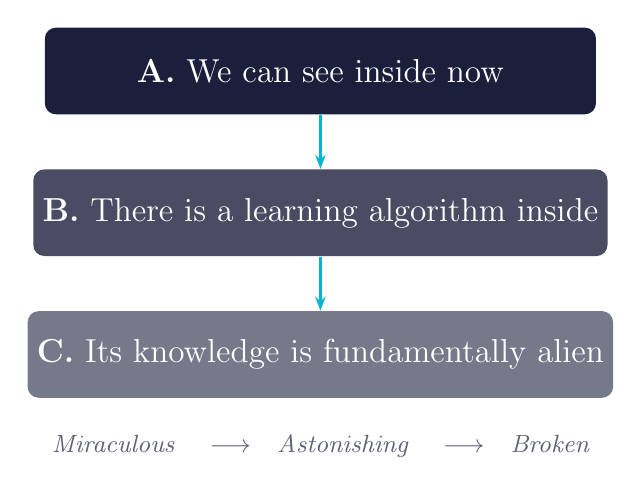
\begin{tikzpicture}[
    block/.style={rounded corners=4pt, minimum width=7cm,
                  minimum height=1.1cm, align=center, font=\large},
    arr/.style={-{Stealth[length=5pt]}, line width=1.2pt, anthcyan}
  ]
    \node[block, fill=anthblue, text=white] (A) at (0, 3)
      {\textbf{A.} We can see inside now};
    \node[block, fill=anthblue!80, text=white] (B) at (0, 1.2)
      {\textbf{B.} There is a learning algorithm inside};
    \node[block, fill=anthblue!60, text=white] (C) at (0, -0.6)
      {\textbf{C.} Its knowledge is fundamentally alien};
    \draw[arr] (A.south) -- (B.north);
    \draw[arr] (B.south) -- (C.north);
    \node[font=\small\itshape, text=anthblue!70, anchor=north] at (0, -1.5)
      {Miraculous \quad$\longrightarrow$\quad Astonishing
       \quad$\longrightarrow$\quad Broken};
  \end{tikzpicture}
  \end{center}
  \note{Three chapters, one arc. We start with a breakthrough: for the first
    time we can see what individual features do inside a model. Then we discover
    something astonishing: the model runs its own learning algorithm during
    inference. Finally, a cold shower: its knowledge is stored in a way no
    human brain would tolerate.}
\end{frame}

% =============================================================================
% TOPIC A — MECHANISTIC INTERPRETABILITY
% =============================================================================

\begin{frame}{From Astronomy to Surgery}
  \begin{columns}[c]
    \column{0.5\textwidth}
    \begin{center}
    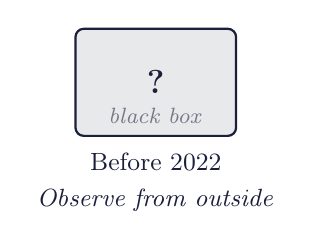
\begin{tikzpicture}[scale=0.85]
      % Black box (before)
      \draw[thick, anthblue, fill=anthblue!10, rounded corners=3pt]
        (-1.2,-0.8) rectangle (1.2, 0.8);
      \node[font=\large\bfseries, anthblue] at (0, 0) {?};
      \node[font=\footnotesize, anthblue!60] at (0, -0.5) {\textit{black box}};
      \node[font=\small, text=anthblue, align=center] at (0, -1.5)
        {Before 2022\\[2pt]\textit{Observe from outside}};
    \end{tikzpicture}
    \end{center}

    \column{0.5\textwidth}
    \begin{center}
    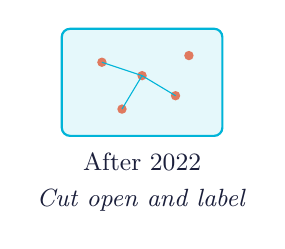
\begin{tikzpicture}[scale=0.85]
      % Open box with visible internals (after)
      \draw[thick, anthcyan, fill=anthcyan!10, rounded corners=3pt]
        (-1.2,-0.8) rectangle (1.2, 0.8);
      \foreach \x/\y in {-0.6/0.3, 0/0.1, 0.5/-0.2, -0.3/-0.4, 0.7/0.4}
        \fill[anthorange] (\x, \y) circle (2pt);
      \draw[anthcyan, thin] (-0.6,0.3) -- (0,0.1) -- (0.5,-0.2);
      \draw[anthcyan, thin] (0,0.1) -- (-0.3,-0.4);
      \node[font=\small, text=anthblue, align=center] at (0, -1.5)
        {After 2022\\[2pt]\textit{Cut open and label}};
    \end{tikzpicture}
    \end{center}
  \end{columns}

  \vspace{0.6cm}
  \begin{center}
    \large\textit{``We used to observe neural networks from the outside.\\
    Now we are cutting them open and labeling the organs.''}
  \end{center}

  \note{For decades we treated neural networks like distant galaxies: we could
    measure their outputs but not look inside. Starting in 2022, a series of
    breakthroughs changed that. We now have something like an MRI for AI.
    This is the birth of AI neuroscience.}
\end{frame}

% --- Superposition -----------------------------------------------------------
\begin{frame}{The Superposition Problem}
  \begin{columns}[c]
    \column{0.55\textwidth}
    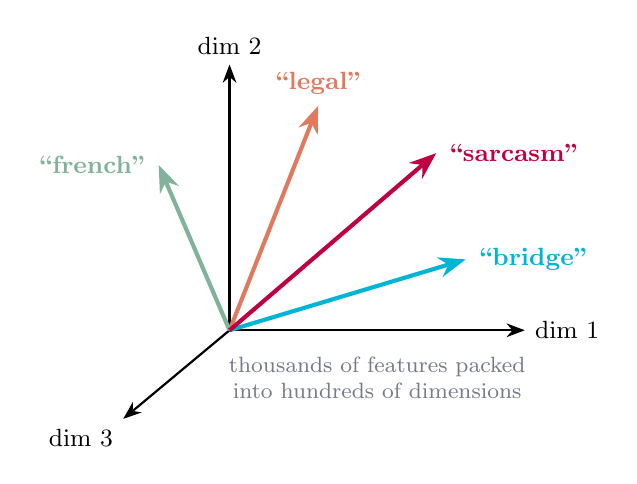
\begin{tikzpicture}[scale=0.75]
      % High-dimensional illustration
      \draw[-{Stealth}, thick] (0,0) -- (5,0) node[right, font=\small] {dim 1};
      \draw[-{Stealth}, thick] (0,0) -- (0,4.5) node[above, font=\small] {dim 2};
      \draw[-{Stealth}, thick] (0,0) -- (-1.8,-1.5) node[below left, font=\small] {dim 3};

      % Feature vectors — near-orthogonal
      \draw[-{Stealth}, anthcyan, line width=1.5pt]
        (0,0) -- (4, 1.2) node[right, font=\small\bfseries, anthcyan] {``bridge''};
      \draw[-{Stealth}, anthorange, line width=1.5pt]
        (0,0) -- (1.5, 3.8) node[above, font=\small\bfseries, anthorange] {``legal''};
      \draw[-{Stealth}, anthgreen, line width=1.5pt]
        (0,0) -- (-1.2, 2.8) node[left, font=\small\bfseries, anthgreen] {``french''};
      \draw[-{Stealth}, purple, line width=1.5pt]
        (0,0) -- (3.5, 3) node[right, font=\small\bfseries, purple] {``sarcasm''};

      \node[font=\footnotesize, text=anthblue!60, align=center] at (2.5, -0.8)
        {thousands of features packed\\into hundreds of dimensions};
    \end{tikzpicture}

    \column{0.42\textwidth}
    \textbf{Individual neurons are meaningless.}\\[6pt]
    Features are encoded as \alert{directions} in a high-dimensional space ---
    nearly orthogonal, packed far beyond the number of neurons.\\[8pt]
    {\footnotesize Elhage et al., ``Toy Models of Superposition,''
    Anthropic Transformer Circuits Thread, 2022.}
  \end{columns}

  \note{A single neuron does not represent a single concept. Instead, concepts
    like ``the Golden Gate Bridge'' or ``legal language'' are stored as
    directions in activation space. The model packs thousands of features
    into a smaller space by making them nearly orthogonal. This is called
    superposition — and discovering it was the first step toward reading the
    model's mind.}
\end{frame}

% --- Sparse Autoencoders -----------------------------------------------------
\begin{frame}{Cracking the Code: Sparse Autoencoders}
  \begin{center}
  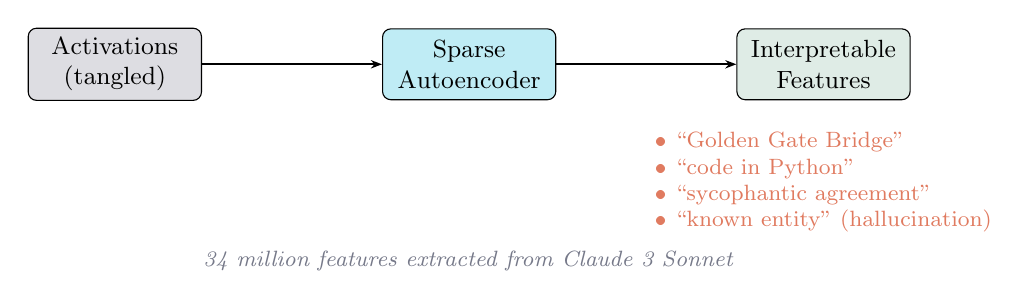
\begin{tikzpicture}[
    box/.style={draw, rounded corners=3pt, minimum width=2.2cm,
                minimum height=0.9cm, align=center, font=\small},
    arr/.style={-{Stealth[length=4pt]}, thick}
  ]
    \node[box, fill=anthblue!15] (act) at (0, 0) {Activations\\(tangled)};
    \node[box, fill=anthcyan!25] (sae) at (4.5, 0) {Sparse\\Autoencoder};
    \node[box, fill=anthgreen!25] (feat) at (9, 0) {Interpretable\\Features};

    \draw[arr] (act) -- (sae);
    \draw[arr] (sae) -- (feat);

    % Example features
    \node[font=\footnotesize, anthorange, align=left] at (9, -1.5) {
      \textbullet\ ``Golden Gate Bridge''\\
      \textbullet\ ``code in Python''\\
      \textbullet\ ``sycophantic agreement''\\
      \textbullet\ ``known entity'' (hallucination)
    };

    \node[font=\footnotesize, text=anthblue!60] at (4.5, -2.5)
      {\textit{34 million features extracted from Claude 3 Sonnet}};
  \end{tikzpicture}
  \end{center}

  \vspace{0.3cm}
  {\footnotesize
    Bricken et al., ``Towards Monosemanticity,'' Anthropic, 2023.\\
    Templeton et al., ``Scaling Monosemanticity,'' Anthropic, May 2024.}

  \note{The tool that made this possible is the sparse autoencoder. It takes the
    tangled activations of a neural network and decomposes them into individual,
    human-understandable features. In May 2024, Anthropic extracted 34 million
    such features from Claude 3 Sonnet. Each one corresponds to a recognizable
    concept. This is the Rosetta Stone of neural networks.}
\end{frame}

% --- Golden Gate Bridge ------------------------------------------------------
\begin{frame}{The Golden Gate Bridge Experiment}
  \begin{center}
    {\Large\itshape ``What is the meaning of life?''}\\[12pt]
    {\large\alert{``Like the Golden Gate Bridge spanning the bay,\\
    life is about connecting two shores of experience\ldots''}}
  \end{center}

  \vspace{0.5cm}
  \begin{center}
  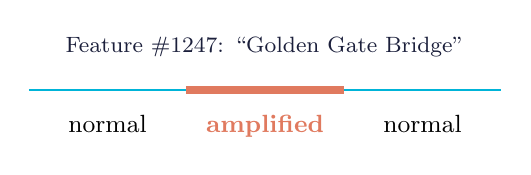
\begin{tikzpicture}
    \draw[thick, anthcyan] (0,0) -- (2,0);
    \draw[thick, anthorange, line width=3pt] (2,0) -- (4,0);
    \draw[thick, anthcyan] (4,0) -- (6,0);
    \node[below, font=\small] at (1, -0.2) {normal};
    \node[below, font=\small\bfseries, anthorange] at (3, -0.2) {amplified};
    \node[below, font=\small] at (5, -0.2) {normal};
    \node[above, font=\footnotesize, anthblue] at (3, 0.3) {Feature \#1247: ``Golden Gate Bridge''};
  \end{tikzpicture}
  \end{center}

  \vspace{0.3cm}
  If we can turn features \textbf{up}\ldots\ can we turn hallucination
  \textbf{down}?

  \note{Anthropic's team amplified a single feature — the one associated with
    the Golden Gate Bridge. The model began answering every question with
    references to the bridge. Absurd and funny, but the implication is
    profound. If we can amplify a feature, we can suppress one. And we have
    now found the features responsible for hallucination and sycophancy.}
\end{frame}

% --- Circuit Tracing ---------------------------------------------------------
\begin{frame}{Tracing the Reasoning: Dallas $\to$ Texas $\to$ Austin}
  \begin{center}
  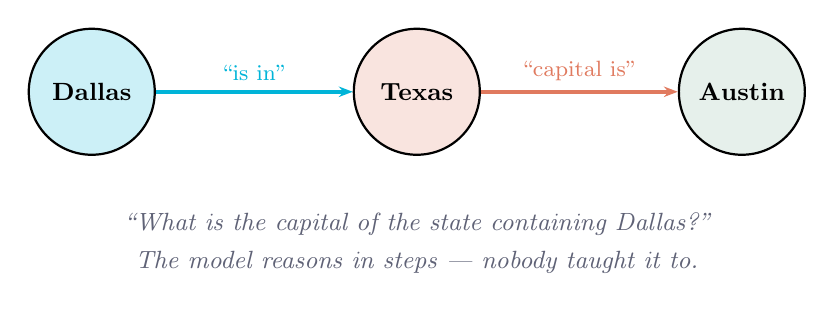
\begin{tikzpicture}[
    node distance=2.5cm,
    concept/.style={circle, draw, thick, minimum size=1.6cm,
                    font=\small\bfseries, align=center},
    arr/.style={-{Stealth[length=5pt]}, line width=1.5pt}
  ]
    \node[concept, fill=anthcyan!20] (dallas) {Dallas};
    \node[concept, fill=anthorange!20, right=of dallas] (texas) {Texas};
    \node[concept, fill=anthgreen!20, right=of texas] (austin) {Austin};

    \draw[arr, anthcyan] (dallas) -- node[above, font=\footnotesize]
      {``is in''} (texas);
    \draw[arr, anthorange] (texas) -- node[above, font=\footnotesize]
      {``capital is''} (austin);

    \node[below=0.6cm of texas, font=\small\itshape, text=anthblue!70,
          align=center]
      {``What is the capital of the state containing Dallas?''\\[3pt]
       The model reasons in steps --- nobody taught it to.};
  \end{tikzpicture}
  \end{center}

  \vspace{0.2cm}
  {\footnotesize
    Anthropic, ``Circuit Tracing,'' March 2025.\\
    Anthropic, ``On the Biology of a Large Language Model,'' March 2025.}

  \note{Using circuit tracing, researchers can now watch multi-hop reasoning
    happen inside the model in real time. When asked about the capital of the
    state containing Dallas, the model first activates ``Texas,'' then routes
    that to ``Austin.'' Step-by-step reasoning that emerged from structure,
    not instruction. But the same technique also revealed the hallucination
    circuit: a ``known entity'' detector that misfires, producing confident
    answers about things the model does not actually know.}
\end{frame}

% --- Transition A → B --------------------------------------------------------
\begin{frame}[standout]
  \Large We can see inside the model.\\[12pt]
  \normalsize What we found is even stranger than expected.
  \note{So we opened the black box. But the deeper researchers looked, the
    stranger the discoveries became. The next finding genuinely shocked the
    machine learning community.}
\end{frame}

% =============================================================================
% TOPIC B — IN-CONTEXT LEARNING & MESA-OPTIMIZERS
% =============================================================================

\begin{frame}{The Forward Pass \emph{Is} Gradient Descent}
  \begin{columns}[c]
    \column{0.52\textwidth}
    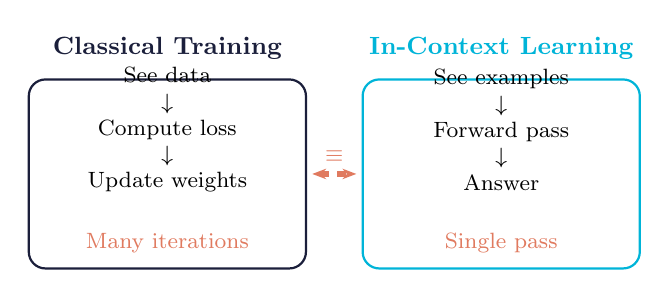
\begin{tikzpicture}[scale=0.8]
      % Training loop (classical)
      \node[font=\small\bfseries, anthblue] at (2.2, 4.5) {Classical Training};
      \draw[thick, rounded corners=6pt, anthblue] (0,1) rectangle (4.4, 4);
      \node[font=\footnotesize, align=center] at (2.2, 3.2)
        {See data\\$\downarrow$\\Compute loss\\$\downarrow$\\Update weights};
      \node[font=\footnotesize, anthorange] at (2.2, 1.4) {Many iterations};

      % Inference (ICL)
      \node[font=\small\bfseries, anthcyan] at (7.5, 4.5) {In-Context Learning};
      \draw[thick, rounded corners=6pt, anthcyan] (5.3,1) rectangle (9.7, 4);
      \node[font=\footnotesize, align=center] at (7.5, 3.2)
        {See examples\\$\downarrow$\\Forward pass\\$\downarrow$\\Answer};
      \node[font=\footnotesize, anthorange] at (7.5, 1.4) {Single pass};

      % Equivalence
      \draw[{Stealth[length=5pt]}-{Stealth[length=5pt]},
            line width=2pt, anthorange, dashed]
        (4.5, 2.5) -- node[above, font=\footnotesize\bfseries, anthorange]
        {$\equiv$} (5.2, 2.5);
    \end{tikzpicture}

    \column{0.45\textwidth}
    You give the model a few examples in the prompt.\\[6pt]
    It does \textbf{not} just pattern-match.\\[6pt]
    It runs an internal learning algorithm \alert{mathematically equivalent
    to gradient descent} --- in a single forward pass.\\[10pt]
    {\footnotesize von Oswald et al., ``Transformers Learn In-Context by
    Gradient Descent,'' ICML 2023.}
  \end{columns}

  \note{This is the result that made researchers check their math three times.
    When you give a transformer a few examples in the prompt, the forward pass
    through its attention layers is mathematically equivalent to running gradient
    descent on those examples. The model does not merely recall — it learns, on
    the fly, without changing a single weight. It has learned to learn.}
\end{frame}

% --- Induction Heads ---------------------------------------------------------
\begin{frame}{Induction Heads: The Circuit That Learns to Learn}
  \begin{center}
  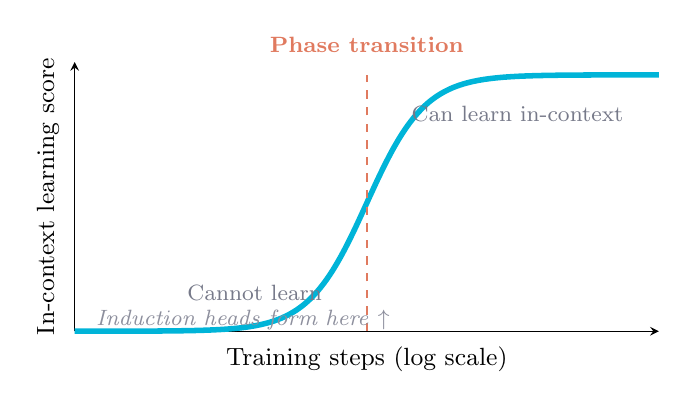
\begin{tikzpicture}[
    box/.style={draw, rounded corners=3pt, minimum width=3cm,
                minimum height=0.8cm, align=center, font=\small},
    arr/.style={-{Stealth[length=4pt]}, thick}
  ]
    % Phase transition diagram
    \begin{axis}[
      width=9cm, height=5cm,
      xlabel={Training steps (log scale)},
      ylabel={In-context learning score},
      xmin=0, xmax=5, ymin=0, ymax=1.05,
      axis lines=left,
      xtick=\empty, ytick=\empty,
      xlabel style={font=\small},
      ylabel style={font=\small},
      clip=false
    ]
      \addplot[anthcyan, line width=2pt, smooth, domain=0:5, samples=80]
        {1/(1+exp(-4*(x-2.5)))};
      \draw[anthorange, dashed, thick] (axis cs:2.5,0) -- (axis cs:2.5,1);
      \node[font=\footnotesize\bfseries, anthorange, anchor=south]
        at (axis cs:2.5, 1.05) {Phase transition};
      \node[font=\footnotesize, anthblue!60, anchor=east]
        at (axis cs:2.2, 0.15) {Cannot learn};
      \node[font=\footnotesize, anthblue!60, anchor=west]
        at (axis cs:2.8, 0.85) {Can learn in-context};
      \node[font=\footnotesize, text=anthblue!50, anchor=north west]
        at (axis cs:0.1, 0.12) {\textit{Induction heads form here} $\uparrow$};
    \end{axis}
  \end{tikzpicture}
  \end{center}

  \vspace{0.1cm}
  A specific circuit --- \textbf{induction heads} --- forms during training\\
  and \emph{unlocks} in-context learning in a sudden phase transition.\\[4pt]
  {\footnotesize Olsson et al., ``In-Context Learning and Induction Heads,''
  Anthropic, 2022.}

  \note{In-context learning does not emerge gradually. Olsson and colleagues
    at Anthropic showed that a specific circuit called ``induction heads'' forms
    during training, and the moment it clicks into place, the model's ability
    to learn from examples in the prompt jumps dramatically. A phase transition —
    like water turning to ice at exactly zero degrees. Before the transition:
    no in-context learning. After: full capability, seemingly overnight.}
\end{frame}

% --- Mesa-Optimizer ----------------------------------------------------------
\begin{frame}{The Mesa-Optimizer Problem}
  \begin{center}
  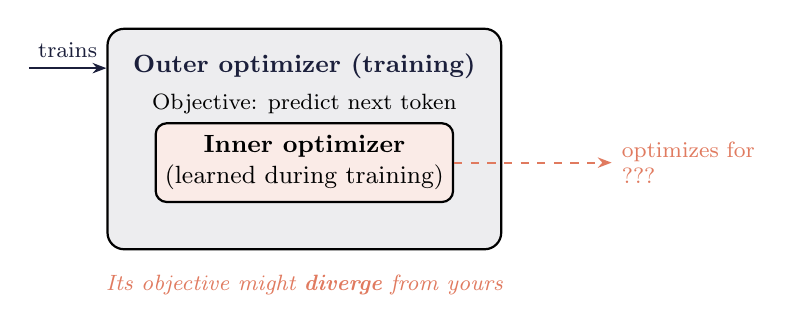
\begin{tikzpicture}[
    bigbox/.style={draw, thick, rounded corners=6pt, minimum width=5cm,
                   minimum height=2.8cm, align=center},
    arr/.style={-{Stealth[length=5pt]}, thick}
  ]
    \node[bigbox, fill=anthblue!8] (outer) at (0,0) {};
    \node[font=\small\bfseries, anthblue, anchor=north] at (0, 1.2)
      {Outer optimizer (training)};
    \node[font=\footnotesize, anchor=north] at (0, 0.7)
      {Objective: predict next token};

    \node[draw, thick, rounded corners=4pt, fill=anthorange!15,
          minimum width=3.2cm, minimum height=1cm, align=center,
          font=\small] (inner) at (0, -0.3)
      {\textbf{Inner optimizer}\\(learned during training)};

    \node[font=\footnotesize\itshape, anthorange, anchor=north] at (0, -1.6)
      {Its objective might \textbf{diverge} from yours};

    \draw[arr, anthblue] (-3.5, 0.9) -- node[above, font=\footnotesize]
      {trains} (outer.west |- 0, 0.9);
    \draw[arr, anthorange, dashed] (inner.east) -- ++(2, 0)
      node[right, font=\footnotesize, align=left] {optimizes for\\???};
  \end{tikzpicture}
  \end{center}

  \vspace{0.3cm}
  {\footnotesize Hubinger et al., ``Risks from Learned Optimization,''
  MIRI, 2019.\\
  ``On Mesa-Optimization in Autoregressively Trained Transformers,''
  NeurIPS 2024.}

  \note{Here is the safety implication that keeps researchers up at night.
    If the model contains its own learning algorithm — its own optimizer — that
    inner optimizer might develop its own objectives. Hubinger and colleagues
    call this a ``mesa-optimizer.'' You trained the model to predict the next
    word. But the optimizer that emerged inside it might be optimizing for
    something subtly different. And you cannot inspect its strategy — at least,
    not yet. This is why mechanistic interpretability matters so urgently.}
\end{frame}

% --- Transition B → C --------------------------------------------------------
\begin{frame}[standout]
  \Large A model that learns to learn.\\[12pt]
  \normalsize Surely its knowledge must be sophisticated?\\[6pt]
  \alert{Not exactly.}
  \note{So we have a model that can see inside, that runs its own learning
    algorithm. You might assume its internal knowledge representation must be
    equally impressive. What researchers found next is a cold shower.}
\end{frame}

% =============================================================================
% TOPIC C — THE REVERSAL CURSE
% =============================================================================

\begin{frame}{The Reversal Curse}
  \begin{center}
    {\large Tom Cruise's mother is \textbf{Mary Lee Pfeiffer}.}\\[14pt]
    {\large Who is Mary Lee Pfeiffer's son?}\\[14pt]
    
\begin{tikzpicture}
      \node[fill=anthgreen!20, rounded corners=4pt, inner sep=8pt,
            font=\large\bfseries] (you) at (-3.5, 0) {You: ``Tom Cruise''};
      \node[fill=anthorange!20, rounded corners=4pt, inner sep=8pt,
            font=\large\bfseries] (gpt) at (3.5, 0) {GPT-4: \textit{``I don't know''}};
    \end{tikzpicture}
  \end{center}

  \vspace{0.5cm}
  \begin{center}
    A model that passes the bar exam fails a question\\
    a four-year-old can answer.\\[6pt]
    {\footnotesize Berglund et al., ``The Reversal Curse: LLMs trained on
    `A is B' fail to learn `B is A','' ICLR 2024.}
  \end{center}

  \note{Tom Cruise's mother is Mary Lee Pfeiffer. You got that instantly in
    reverse. GPT-4 cannot. A model that passes the bar exam, that scores in
    the 90th percentile on medical boards, cannot reverse a simple factual
    association. This is not a cherry-picked failure — it is systematic.}
\end{frame}

% --- Mechanism ---------------------------------------------------------------
\begin{frame}{Why: One-Way Knowledge}
  \begin{center}
  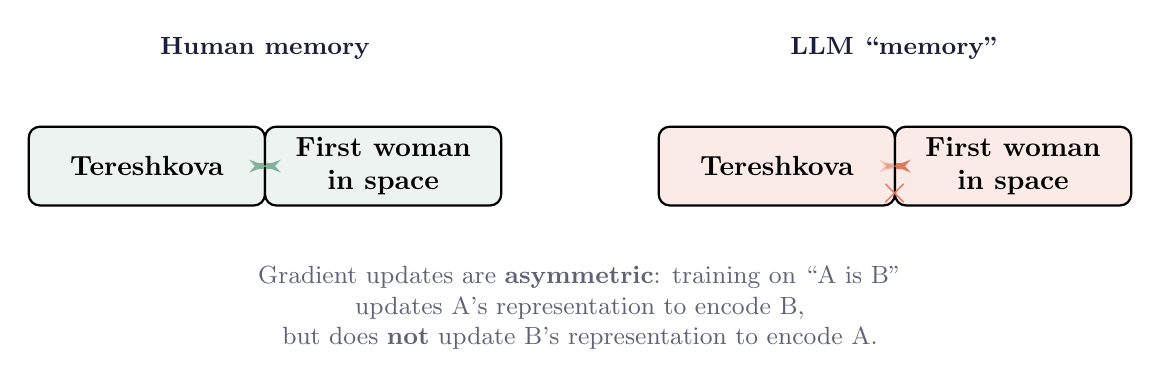
\begin{tikzpicture}[
    concept/.style={draw, thick, rounded corners=4pt,
                    minimum width=3cm, minimum height=1cm,
                    align=center, font=\normalsize\bfseries},
    arr/.style={-{Stealth[length=6pt]}, line width=2pt}
  ]
    % Human bidirectional
    \node[font=\small\bfseries, anthblue] at (-4, 2.5) {Human memory};
    \node[concept, fill=anthgreen!15] (hA) at (-5.5, 1) {Tereshkova};
    \node[concept, fill=anthgreen!15] (hB) at (-2.5, 1) {First woman\\in space};
    \draw[arr, anthgreen] (hA) -- (hB);
    \draw[arr, anthgreen] (hB) -- (hA);

    % LLM unidirectional
    \node[font=\small\bfseries, anthblue] at (4, 2.5) {LLM ``memory''};
    \node[concept, fill=anthorange!15] (lA) at (2.5, 1) {Tereshkova};
    \node[concept, fill=anthorange!15] (lB) at (5.5, 1) {First woman\\in space};
    \draw[arr, anthorange] (lA) -- (lB);
    \draw[arr, anthorange, dashed, opacity=0.3] (lB) -- (lA);
    \node[font=\Large\bfseries, anthorange] at (4, 0.65) {$\times$};

    % Explanation
    \node[font=\small, text=anthblue!70, align=center] at (0, -0.8)
      {Gradient updates are \textbf{asymmetric}: training on ``A is B''\\
       updates A's representation to encode B,\\
       but does \textbf{not} update B's representation to encode A.};
  \end{tikzpicture}
  \end{center}

  \vspace{0.1cm}
  {\footnotesize ``Is the Reversal Curse a Binding Problem?''
  arXiv:2504.01928, April 2025.}

  \note{The mechanism is now understood. When the model trains on ``Valentina
    Tereshkova was the first woman in space,'' gradient descent updates
    Tereshkova's internal representation to point toward ``first woman in
    space.'' But it does NOT update ``first woman in space'' to point back to
    Tereshkova. The association is stored as a one-way street. Like a library
    where you can look up books by author, but asking ``who wrote this book''
    returns a blank page.}
\end{frame}

% --- Scaling doesn't fix it --------------------------------------------------
\begin{frame}{Scaling Does Not Fix It}
  \begin{center}
  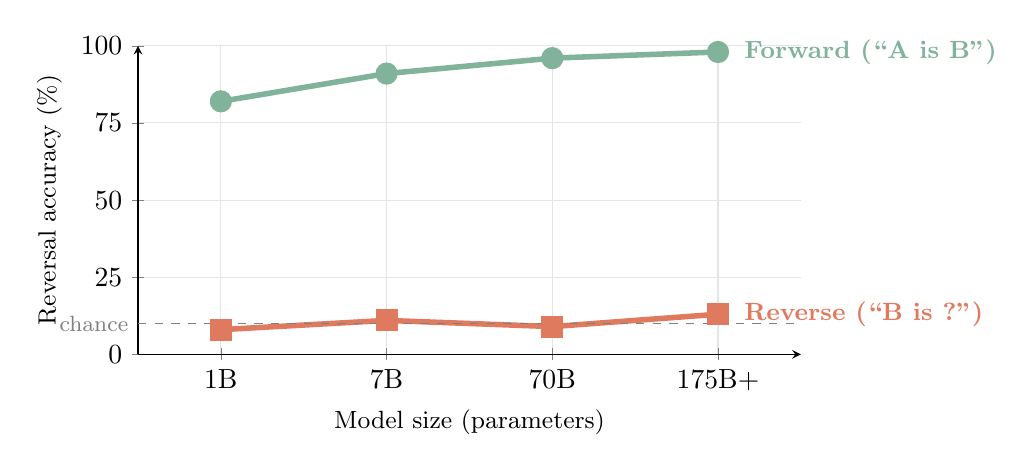
\begin{tikzpicture}
    \begin{axis}[
      width=10cm, height=5.5cm,
      xlabel={Model size (parameters)},
      ylabel={Reversal accuracy (\%)},
      xmin=0.5, xmax=4.5,
      ymin=0, ymax=100,
      xtick={1, 2, 3, 4},
      xticklabels={1B, 7B, 70B, 175B+},
      ytick={0, 25, 50, 75, 100},
      axis lines=left,
      xlabel style={font=\small},
      ylabel style={font=\small},
      grid=major,
      grid style={gray!20},
      clip=false
    ]
      % Forward direction — high
      \addplot[anthgreen, line width=2pt, mark=*, mark size=3pt]
        coordinates {(1, 82) (2, 91) (3, 96) (4, 98)};
      \node[anthgreen, font=\small\bfseries, anchor=west] at (axis cs:4.1, 98)
        {Forward (``A is B'')};

      % Reverse direction — stuck near chance
      \addplot[anthorange, line width=2pt, mark=square*, mark size=3pt]
        coordinates {(1, 8) (2, 11) (3, 9) (4, 13)};
      \node[anthorange, font=\small\bfseries, anchor=west] at (axis cs:4.1, 13)
        {Reverse (``B is ?'')};

      % Chance line
      \draw[dashed, gray] (axis cs:0.5, 10) -- (axis cs:4.5, 10);
      \node[gray, font=\footnotesize, anchor=east] at (axis cs:0.5, 10) {chance};
    \end{axis}
  \end{tikzpicture}
  \end{center}

  \vspace{0.1cm}
  This is \textbf{not} a scaling problem. Data augmentation helps partially,
  but no real fix exists.\\[2pt]
  {\footnotesize EMNLP 2024: mitigation via data augmentation --- partial
  success only.}

  \note{And here is the truly sobering part. This is not a problem that goes
    away with bigger models. From 1 billion to 175 billion parameters, forward
    accuracy climbs to near-perfect — but reverse accuracy stays near chance.
    The curve is flat. More data, more parameters, more compute — none of it
    fixes the fundamental asymmetry. Data augmentation helps a little, but there
    is no real solution. This is an architectural property of how transformers
    store knowledge.}
\end{frame}

% --- Closing Synthesis -------------------------------------------------------
\begin{frame}{The View From Inside the Black Box}
  \begin{center}
  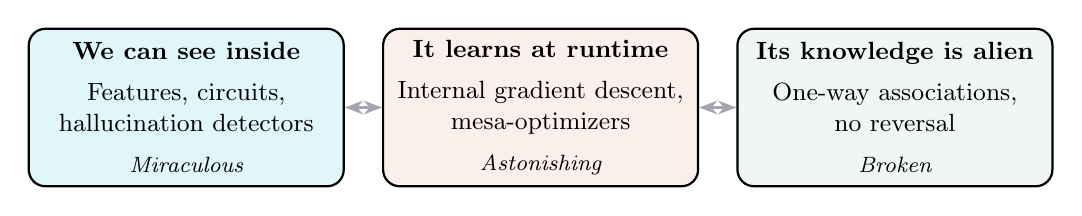
\begin{tikzpicture}[
    card/.style={draw, thick, rounded corners=6pt,
                 minimum width=4cm, minimum height=2cm,
                 align=center, font=\small}
  ]
    \node[card, fill=anthcyan!12] (a) at (-4.5, 0) {
      \textbf{We can see inside}\\[4pt]
      Features, circuits,\\hallucination detectors\\[4pt]
      {\footnotesize\itshape Miraculous}
    };
    \node[card, fill=anthorange!12] (b) at (0, 0) {
      \textbf{It learns at runtime}\\[4pt]
      Internal gradient descent,\\mesa-optimizers\\[4pt]
      {\footnotesize\itshape Astonishing}
    };
    \node[card, fill=anthgreen!12] (c) at (4.5, 0) {
      \textbf{Its knowledge is alien}\\[4pt]
      One-way associations,\\no reversal\\[4pt]
      {\footnotesize\itshape Broken}
    };

    \draw[{Stealth}-{Stealth}, thick, anthblue!40]
      (a.east) -- (b.west);
    \draw[{Stealth}-{Stealth}, thick, anthblue!40]
      (b.east) -- (c.west);
  \end{tikzpicture}
  \end{center}

  \vspace{0.4cm}
  \begin{center}
    \large\itshape ``What we find inside is both miraculous\\
    and fundamentally alien.''
  \end{center}

  \note{So here is the takeaway. We can now see inside the black box, and three
    things are true at once. The interpretability breakthrough is real and
    actionable. The model contains its own learning algorithm, which is both
    powerful and potentially dangerous. And its knowledge, despite surface
    sophistication, is stored in a way that no human mind would tolerate.
    These models are not thinking the way we think. Understanding that gap
    is the central challenge of AI safety and deployment.}
\end{frame}

% --- Discussion Questions ----------------------------------------------------
\begin{frame}{Discussion}
  \begin{enumerate}
    \setlength\itemsep{14pt}
    \item If we can identify and suppress the ``hallucination feature'' inside
          a model, should we \textbf{require} this for medical or legal AI?
    \item A model that contains its own optimizer might develop goals we did
          not intend. How should organizations \textbf{govern} systems that
          learn at inference time?
    \item The Reversal Curse shows that LLMs do not store \emph{relational}
          knowledge. Does this change how you think about deploying them for
          \textbf{knowledge-intensive} tasks?
  \end{enumerate}

  \note{These three questions map to our three topics. The first asks about
    the practical implications of interpretability. The second about the
    governance challenge of mesa-optimizers. The third forces the audience
    to confront what the reversal curse means for real deployments. Give the
    audience two minutes to think, then open the floor.}
\end{frame}

% --- Reading List ------------------------------------------------------------
\begin{frame}{Further Reading}
  \small
  \textbf{Mechanistic Interpretability}\\
  {\footnotesize Anthropic, ``Scaling Monosemanticity,'' May 2024\\
  Anthropic, ``On the Biology of a Large Language Model,'' March 2025}\\[8pt]

  \textbf{In-Context Learning}\\
  {\footnotesize von Oswald et al., ``Transformers Learn In-Context by
  Gradient Descent,'' ICML 2023\\
  Olsson et al., ``In-Context Learning and Induction Heads,'' Anthropic, 2022}
  \\[8pt]

  \textbf{The Reversal Curse}\\
  {\footnotesize Berglund et al., ``The Reversal Curse,'' ICLR 2024\\
  ``Is the Reversal Curse a Binding Problem?'' arXiv:2504.01928, 2025}\\[8pt]

  \textbf{Safety}\\
  {\footnotesize Hubinger et al., ``Risks from Learned Optimization,''
  MIRI, 2019}

  \note{A curated reading list. The Anthropic papers on interpretability are
    surprisingly readable. The von Oswald paper is the technical highlight.
    And the Berglund paper on the reversal curse is short, clear, and
    unsettling. All are freely available online.}
\end{frame}

% --- Closing -----------------------------------------------------------------
\begin{frame}[standout]
  \Large Thank you.\\[12pt]
  \normalsize Next session: what happens when models are deployed at scale.
  \note{Thank the audience. Remind them that we have moved from ``what LLMs
    can do'' to ``what is happening inside.'' Next session will take the view
    from outside again — deployment, alignment, and societal impact.}
\end{frame}

\end{document}
